% Drawing 58/03-2 -- folder 58, batch 03, archive page 56 (PDF page 57).
% Transcription: à droite : un quadrant d'axes $p$ (horizontal) et $q$ (vertical) couvert de droites obliques parallèles montant vers la droite ; légendes : en haut à gauche « \ill{} » et « $q$ », à droite « $p$ » et « \uncertain{filtre} » ; quelques points isolés à droite.
% Kind: quadrant covered with parallel oblique lines. Method 2 (schematic redraw from the facsimile). Status: partial.
% Notes: The two axes (the vertical one is doubled on the page: drawn once), eight parallel oblique strokes rising to the right, the first three starting on the vertical axis and the others on the horizontal axis, and the labels q (top of the vertical axis), p and the word read « filtre » by the transcription (uncertain there; kept) at the right; the illegible word at the upper left is left out. Four isolated dots at the right are drawn. Still differs: the strokes are free and not exactly parallel; fainter pencil strokes between them are left out, so the count (eight) is that of the ink strokes as read. Redrawn 2026-11-12 (issue 128): to check again.
% Coordinates: 1 unit = 1 mm = 1/100 of the crop width (bbox in page fractions: [0.54, 0.46, 0.99, 0.71]).
% Redrawn by Claude (claude-fable-5-2), issue #128, 2026-11-12; not checked by a human; not compiled (no TeX in the session).
% Rights: reproduces part of the work -- behind RENDER_TRANSCRIPTS, never published by itself.
\documentclass[tikz,border=3pt]{standalone}
\usepackage{amsmath,amssymb}
\usetikzlibrary{patterns,arrows.meta}
\tikzset{pencil/.style={black!45}, struck/.style={black!35}, mpt/.style={circle,draw,inner sep=1.3pt}, pt/.style={circle,fill,inner sep=0.9pt}, opt/.style={circle,draw,fill=white,inner sep=1.1pt}}
\begin{document}
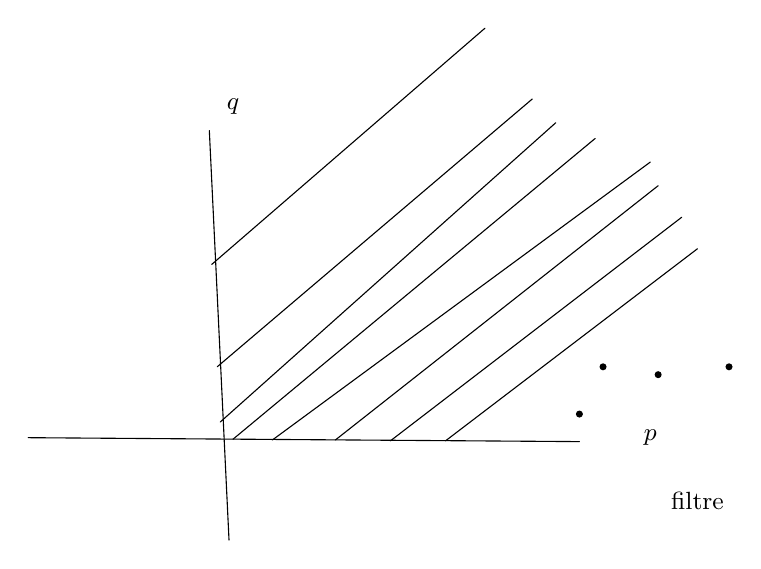
\begin{tikzpicture}[x=1mm,y=1mm,line cap=round,line join=round,font=\scriptsize]
\draw (5,-61) -- (75,-61.5);
\draw (28,-22) -- (30.5,-74);
\draw (28.3,-39) -- (63,-9);
\draw (29,-52) -- (69,-18);
\draw (29.4,-59) -- (72,-21);
\draw (31,-61.2) -- (77,-23);
\draw (36,-61.3) -- (84,-26);
\draw (44,-61.3) -- (85,-29);
\draw (51,-61.4) -- (88,-33);
\draw (58,-61.4) -- (90,-37);
\node[pt] at (78,-52) {};
\node[pt] at (85,-53) {};
\node[pt] at (94,-52) {};
\node[pt] at (75,-58) {};
\node[inner sep=1pt] at (31,-19) {\small $q$};
\node[inner sep=1pt] at (84,-61) {\small $p$};
\node[inner sep=1pt] at (90,-69) {\small filtre};
\end{tikzpicture}
\end{document}
